\chapter{System Architecture}
\label{chap:design_methodology}

This chapter includes a comprehensive review of the design and methods used adopted for developing the AI-driven medical chatbot. The system is tailored to cater to two distinct cohorts: patients and students of medicine, approached from an educational standpoint and pragmatic support including symptom evaluation and independent management of appointments. The complete system flow and design are shown in Figure 3.1.

\section{High-Level Architecture}
\label{sec:high_level_architecture}

The system is structured into several interconnected modules, as shown in Figure.
\begin{figure}[htbp]
    \begin{center}
      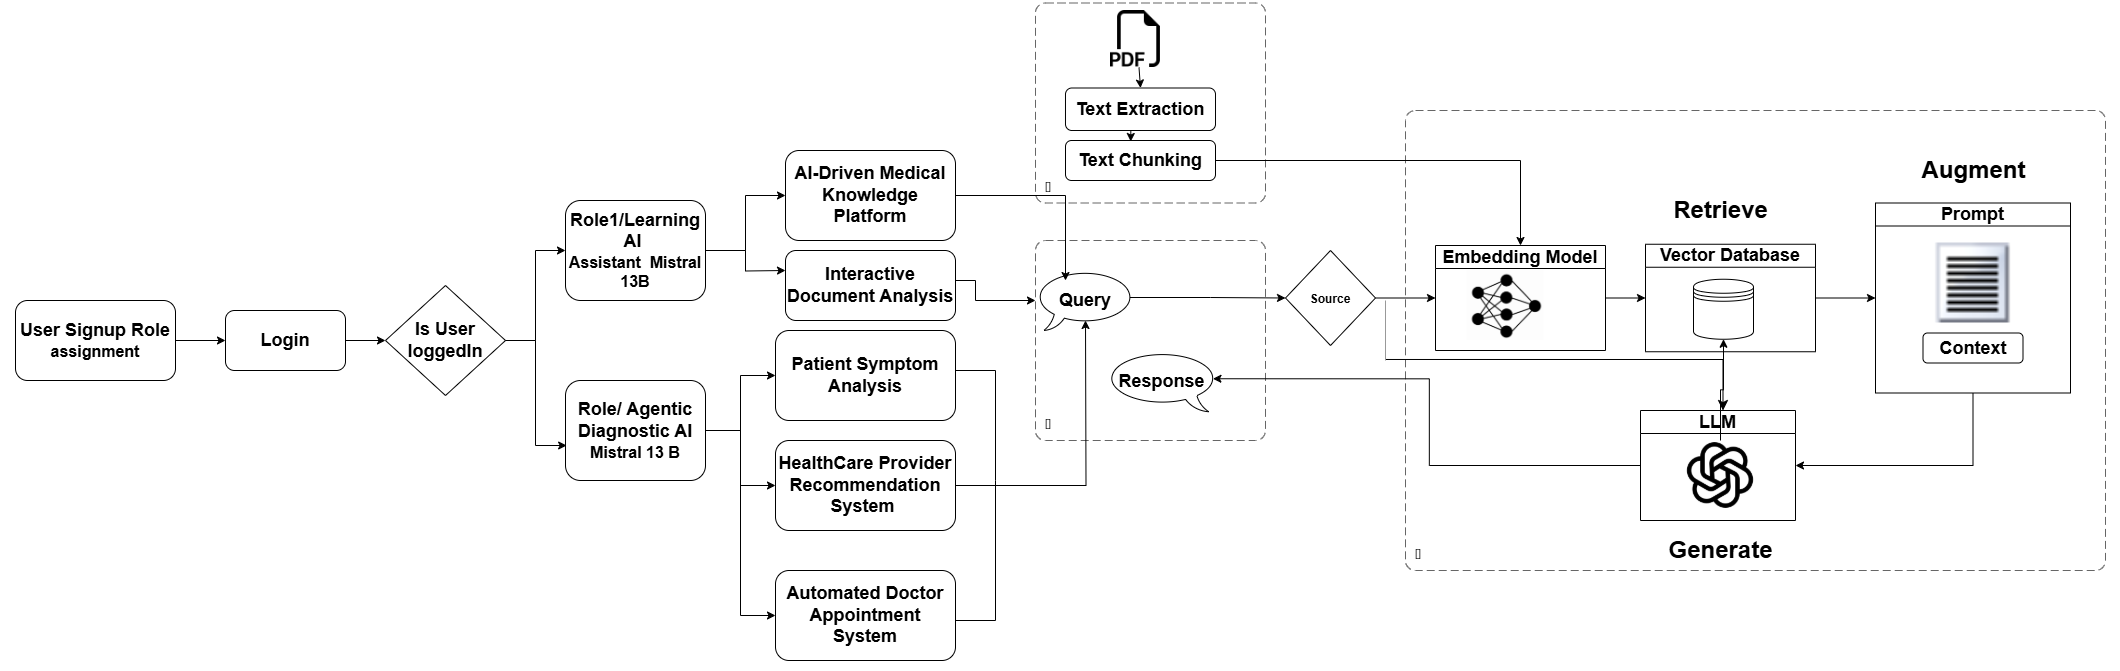
\includegraphics[width=16cm,height=10cm]{./Images/Thesis.png}
       \caption{Thesis implementation phases}
       \label{fig: Thesis implementation phases}
    \end{center}
\end{figure}

\vspace{2cm}
\begin{enumerate}[itemsep=2em]
  \item \textbf{User Authentication and Role Identification:} 
    \begin{itemize}
        \item Upon user login, the system authenticates and decides the individual's role as either medical student or patient.
        \item Role-based access controls the assignment of users to a particular dashboard and capabilities.
    \end{itemize}
  \item \textbf{Role-Based Interaction:} 
    \begin{itemize}
        \item \emph{Medical Student Mode:} Medical Student Mode: Provides exhaustive study aids such as PDF files with scholarly question-and-answer sessions.
        \item \emph{Patient Mode:} Gives a symptom analysis with suggestions for location based doctor recommendation with agentic appointment system.
    \end{itemize}
  \item \textbf{PDF Processing and Text Chunking:} 
    \begin{itemize}
        \item Extracts text from uploaded PDFs and segments them into manageable chunks for embedding and retrieval.
    \end{itemize}
  \item \textbf{Embedding and Vector Storage:}
    \begin{itemize}
        \item Uses \texttt{all-mpnet-base-v2} for semantic embeddings.
        \item Effective similarity-based retrieval depends on stores of embeddings in a vector database (Pinecone).
    \end{itemize}
  \item \textbf{Retrieval-Augmented Generation (RAG):} 
    \begin{itemize}
        \item To get pertinent pieces, user inquiries are incorporated and compared against stored vectors.
        \item Using the \textbf{Mistral 13B Quantized Model}, correct replies are then produced from the recovered context.
    \end{itemize}
  \item \textbf{LLM Response Generation:}
    \begin{itemize}
        \item The Mistral 13B Quantized Model generates context-aware, role-specific answers.
        \item Responses are tailored differently for educational depth (students) and practical advice (patients).
    \end{itemize}
    \vspace{2cm}
  \item \textbf{Agentic Appointment Booking:}
    \begin{itemize}
        \item For patients, the system autonomously schedules appointments by integrating healthcare provider data.
    \end{itemize}
\end{enumerate}

\section{Mistral 13B Quantized Model}
\label{sec:mistral_model}

The \textbf{Mistral 13B Quantized Model} serves as the core LLM for generating responses. It is chosen for its balance between performance and computational efficiency.

\subsection{Overview and Architecture}
\label{subsec:mistral_overview}
The Mistral 13B Quantized Model is a variant of the Mistral architecture known for:
\begin{itemize}[itemsep=2em]
    \item \textbf{Parameter Efficiency:} With 13 billion parameters, it delivers great performance while keeping reasonable resource needs owing to quantization.
    \item \textbf{Quantization Technique:} Uses Q3\_K\_M quantization to rapidly infer without appreciable loss of accuracy by lowering memory footprint.
    \item \textbf{Transformer Architecture:} Built on a decoder-only design with multi-head self-attention and feed-forward layers, tailored for generative workloads, transformer architecture is suited for
\end{itemize}

\subsection{Contextual Response Generation}
\label{subsec:mistral_response}
\begin{itemize}
    \item The model responds using the context obtained from the RAG pipeline.
    \item Role-specific prompts guide the model in generating:
        \begin{itemize}
            \item \emph{Educational Explanations} For medical students with thorough references, educational justifications abound.
            \item Easy, practical advice for patients guarantees clarity and reduces jargon.
        \end{itemize}
\end{itemize}
\vspace{2cm}
\subsection{Role-Specific Prompting}
\label{subsec:mistral_prompting}
Different prompts are crafted based on user roles:
\begin{itemize}[itemsep=2em]
    \item \textbf{For Medical Students:}
        \begin{itemize}
            \item Requests comprehensive explanations with references to academic sources.
            \item Example: “Explain the mechanism of action of beta-blockers with clinical implications.”
        \end{itemize}
    \item \textbf{For Patients:}
        \begin{itemize}
            \item Prompts the model to generate concise, easy-to-understand guidance.
            \item Example: “What should I do if I experience chest pain?”
        \end{itemize}
\end{itemize}

\subsection{Additional Explanation of the Mistral 13B Quantized Model}
\label{subsec:mistral_explanation}
This system has especially selected the Mistral 13B Quantized Model because of its outstanding balance between computational efficiency and high-quality response generating.  Delivering real-time replies in a production setting depends on the model's memory footprint being much reduced by the quantization procedure, which also accelerates inference times.  The model is well-suited for both the exact, practical counsel required by patients and the thorough instructional needs of medical students as it retains strong performance across many tasks despite its small size.


\section{Embedding and Vector Database}
\label{sec:embedding_vector_db}

\subsection{Embedding Model: \texttt{all-mpnet-base-v2}}
\label{subsec:all_mpnet_base_v2}
\text Text chunks and queries are turned into 768-dimensional embeddings using all-mpnet-base-v2.  Important traits consist in:

\begin{itemize}[itemsep=2em]
  \item \textbf{Contextual Semantic Representation:} adds contextual relevance to queries.
  \item \textbf{Performance:} often beats more recent models (such as BERT) in semantic search challenges.
  \item \textbf{Compatibility:} Pinecone stores Embeddings for quick cosine similarity-based searches.
\end{itemize}

\subsection{Vector Database: Pinecone}
\label{subsec:pinecone}
\emph{Pinecone's} flawless integration into the retrieval process and strong performance in maintaining high-dimensional embeddings define it as the vector database.  Important qualities include:

\begin{itemize}[itemsep=2em]
    \item \textbf{Scalability:} Pinecone is made to effectively index and control millions of embeddings, hence guaranteeing low-latency retrieval even as data volume increases.  Applications with fast growing datasets will find this scalability perfect.
    \item \textbf{Metric Support:} Pinecone provides very accurate and significant search results by using cosine similarity as the main measure for relevance ranking; these are vital for guaranteeing that the most contextually relevant information is obtained.
    \item \textbf{High Performance:} The database's performance optimization allows real-time searches and changes.  For uses like the medical chatbot system that need for quick answers, this is absolutely vital.
    \item \textbf{Integration with Retrieval Pipelines:} Pinecone simplifies the process of embedding storage and retrieval by deftly interacting with frameworks like LangChain.  From query embedding to final answer production, this close connection helps to keep a seamless flow.
    \item \textbf{Reliability and Consistency:} For systems managing sensitive and vast data, Pinecone provides a dependable infrastructure guaranteed by durability and consistency of data.
    \item \textbf{Ease of Use:} Pinecone helps developers to construct and run the vector database with little overhead by means of a user-friendly API and strong documentation, therefore promoting quicker development cycles.
\end{itemize}


\section{Agentic Appointment Booking}
\label{sec:agentic_booking}

\subsection{Triggering Conditions and Workflow}
\label{subsec:booking_workflow}
The system autonomously handles appointment booking by:
\begin{enumerate}
    \item Detecting user intent through keywords (e.g., “book an appointment”).
    \item Collecting details like location and specialty.
    \item Generating a booking link via Doctolib and sending it through Twilio SMS integration.
\end{enumerate}

\section{User Interface Approaches}
\label{sec:user_interface}

\subsection{Flask UI}
\label{subsec:flask_ui}
\emph{Flask} is used for:
\begin{itemize}[itemsep=2em]
    \item \textbf{User Authentication:} Role-based access control for students and patients.
    \item \textbf{File Upload:} Allowing PDF uploads for medical students.
    \item \textbf{Query Form:} Basic input form for submitting questions.
\end{itemize}

The Flask UI is made to easily manage file uploads, user registration, and login.  It also links with another Chainlit process with a chat-centric UI.  Successful login causes Flask to launch Chainlit in a fresh thread sending the user's email via environment variables so Chainlit may retrieve role related information from the database.  This connection guarantees that following authentication users are swiftly sent to a dynamic and responsive chatbot interface.


\subsection{Chainlit UI}
\label{subsec:chainlit_ui}
\emph{Chainlit} provides a chat-centric interface designed to enhance user engagement through interactive and dynamic conversation flows. Key features include:
\begin{itemize}[itemsep=2em]
    \item \textbf{Role-Specific Chat Profiles:} The technology lets patients and medical students communicate in numerous ways that fit them.  Whether it implies in-depth academic discussions or simple, attainable health advice, every profile provides customised questions and answers to ensure the conversation remains relevant to the user's situation.
    \item \textbf{Interactive Conversation Elements:} Just a few of the components Chainlit UI offers include real-time feedback, flexible chat threads, and dynamic content loading.  This allows users to interact dynamically with the chatbot since the UI varies depending on user input and inquiry context.
    \item \textbf{Enhanced User Engagement:} Chainlit works to provide an interesting experience by combining interactive buttons and multimedia components.  Users may, for instance, click on recommended subjects or follow-up questions, which simplifies browsing difficult material.
    \item \textbf{Seamless Integration with Back-End Systems:} The UI is made to operate in concert with the underlying retrieval and generating processes. It lets users modify or expand their searches interactively and gets context-aware results from the Mistral 13B Quantized Model that show in an easily consumable way.
    \item \textbf{Customization and Scalability:} Chainlit's modular architecture lets one quickly change chat features and discussion patterns. As new features are included or user demands change, this adaptability helps to promote scalability and continuous improvement.
\end{itemize}

\vspace{5cm}
\section{Summary}
\label{sec:methodology_summary}
This chapter presents in general a strong concept for an artificial intelligence-driven medical chat bot that efficiently serves two different user groups: patients and medical students.  The modular design of the system combines user identification, PDF processing, semantic embedding using all-mpnet-based-v2, and a vector database via Pinecone for fast retrieval.  To provide context-aware replies, a retrieval-augmented generating pipeline deftly combines the potent Mistral 13B Quantized Model.  Moreover, the system offers specific features like autonomous appointment booking and role-based interaction, therefore assuring that practical and instructional demands are both effectively met.  Key component is the way the Chainlit chat interface and the Flask UI are integrated to provide dynamic, real-time interaction using user-specific data to customize answers and services.  The implementation specifics, system deployment, and other integration techniques will cover in the future chapter.


